\documentclass[twoside]{book}

% Packages required by doxygen
\usepackage{fixltx2e}
\usepackage{calc}
\usepackage{doxygen}
\usepackage[export]{adjustbox} % also loads graphicx
\usepackage{graphicx}
\usepackage[utf8]{inputenc}
\usepackage{makeidx}
\usepackage{multicol}
\usepackage{multirow}
\PassOptionsToPackage{warn}{textcomp}
\usepackage{textcomp}
\usepackage[nointegrals]{wasysym}
\usepackage[table]{xcolor}

% Font selection
\usepackage[T1]{fontenc}
\usepackage[scaled=.90]{helvet}
\usepackage{courier}
\usepackage{amssymb}
\usepackage{sectsty}
\renewcommand{\familydefault}{\sfdefault}
\allsectionsfont{%
  \fontseries{bc}\selectfont%
  \color{darkgray}%
}
\renewcommand{\DoxyLabelFont}{%
  \fontseries{bc}\selectfont%
  \color{darkgray}%
}
\newcommand{\+}{\discretionary{\mbox{\scriptsize$\hookleftarrow$}}{}{}}

% Page & text layout
\usepackage{geometry}
\geometry{%
  a4paper,%
  top=2.5cm,%
  bottom=2.5cm,%
  left=2.5cm,%
  right=2.5cm%
}
\tolerance=750
\hfuzz=15pt
\hbadness=750
\setlength{\emergencystretch}{15pt}
\setlength{\parindent}{0cm}
\setlength{\parskip}{3ex plus 2ex minus 2ex}
\makeatletter
\renewcommand{\paragraph}{%
  \@startsection{paragraph}{4}{0ex}{-1.0ex}{1.0ex}{%
    \normalfont\normalsize\bfseries\SS@parafont%
  }%
}
\renewcommand{\subparagraph}{%
  \@startsection{subparagraph}{5}{0ex}{-1.0ex}{1.0ex}{%
    \normalfont\normalsize\bfseries\SS@subparafont%
  }%
}
\makeatother

% Headers & footers
\usepackage{fancyhdr}
\pagestyle{fancyplain}
\fancyhead[LE]{\fancyplain{}{\bfseries\thepage}}
\fancyhead[CE]{\fancyplain{}{}}
\fancyhead[RE]{\fancyplain{}{\bfseries\leftmark}}
\fancyhead[LO]{\fancyplain{}{\bfseries\rightmark}}
\fancyhead[CO]{\fancyplain{}{}}
\fancyhead[RO]{\fancyplain{}{\bfseries\thepage}}
\fancyfoot[LE]{\fancyplain{}{}}
\fancyfoot[CE]{\fancyplain{}{}}
\fancyfoot[RE]{\fancyplain{}{\bfseries\scriptsize Generated by Doxygen }}
\fancyfoot[LO]{\fancyplain{}{\bfseries\scriptsize Generated by Doxygen }}
\fancyfoot[CO]{\fancyplain{}{}}
\fancyfoot[RO]{\fancyplain{}{}}
\renewcommand{\footrulewidth}{0.4pt}
\renewcommand{\chaptermark}[1]{%
  \markboth{#1}{}%
}
\renewcommand{\sectionmark}[1]{%
  \markright{\thesection\ #1}%
}

% Indices & bibliography
\usepackage{natbib}
\usepackage[titles]{tocloft}
\setcounter{tocdepth}{3}
\setcounter{secnumdepth}{5}
\makeindex

% Hyperlinks (required, but should be loaded last)
\usepackage{ifpdf}
\ifpdf
  \usepackage[pdftex,pagebackref=true]{hyperref}
\else
  \usepackage[ps2pdf,pagebackref=true]{hyperref}
\fi
\hypersetup{%
  colorlinks=true,%
  linkcolor=blue,%
  citecolor=blue,%
  unicode%
}

% Custom commands
\newcommand{\clearemptydoublepage}{%
  \newpage{\pagestyle{empty}\cleardoublepage}%
}

\usepackage{caption}
\captionsetup{labelsep=space,justification=centering,font={bf},singlelinecheck=off,skip=4pt,position=top}

%===== C O N T E N T S =====

\begin{document}

% Titlepage & ToC
\hypersetup{pageanchor=false,
             bookmarksnumbered=true,
             pdfencoding=unicode
            }
\pagenumbering{alph}
\begin{titlepage}
\vspace*{7cm}
\begin{center}%
{\Large My Project }\\
\vspace*{1cm}
{\large Generated by Doxygen 1.8.13}\\
\end{center}
\end{titlepage}
\clearemptydoublepage
\pagenumbering{roman}
\tableofcontents
\clearemptydoublepage
\pagenumbering{arabic}
\hypersetup{pageanchor=true}

%--- Begin generated contents ---
\chapter{Hierarchical Index}
\section{Class Hierarchy}
This inheritance list is sorted roughly, but not completely, alphabetically\+:\begin{DoxyCompactList}
\item Mono\+Behaviour\begin{DoxyCompactList}
\item \contentsline{section}{Button\+Manager}{\pageref{class_button_manager}}{}
\item \contentsline{section}{Flipper\+Move}{\pageref{class_flipper_move}}{}
\item \contentsline{section}{Game\+Manager}{\pageref{class_game_manager}}{}
\item \contentsline{section}{Ground\+Points}{\pageref{class_ground_points}}{}
\item \contentsline{section}{Obstacle}{\pageref{class_obstacle}}{}
\item \contentsline{section}{Score}{\pageref{class_score}}{}
\item \contentsline{section}{Spring}{\pageref{class_spring}}{}
\end{DoxyCompactList}
\end{DoxyCompactList}

\chapter{Class Index}
\section{Class List}
Here are the classes, structs, unions and interfaces with brief descriptions\+:\begin{DoxyCompactList}
\item\contentsline{section}{\hyperlink{class_button_manager}{Button\+Manager} }{\pageref{class_button_manager}}{}
\item\contentsline{section}{\hyperlink{class_flipper_move}{Flipper\+Move} }{\pageref{class_flipper_move}}{}
\item\contentsline{section}{\hyperlink{class_game_manager}{Game\+Manager} }{\pageref{class_game_manager}}{}
\item\contentsline{section}{\hyperlink{class_ground_points}{Ground\+Points} }{\pageref{class_ground_points}}{}
\item\contentsline{section}{\hyperlink{class_obstacle}{Obstacle} }{\pageref{class_obstacle}}{}
\item\contentsline{section}{\hyperlink{class_score}{Score} }{\pageref{class_score}}{}
\item\contentsline{section}{\hyperlink{class_spring}{Spring} }{\pageref{class_spring}}{}
\end{DoxyCompactList}

\chapter{Class Documentation}
\hypertarget{class_button_manager}{}\section{Button\+Manager Class Reference}
\label{class_button_manager}\index{Button\+Manager@{Button\+Manager}}
Inheritance diagram for Button\+Manager\+:\begin{figure}[H]
\begin{center}
\leavevmode
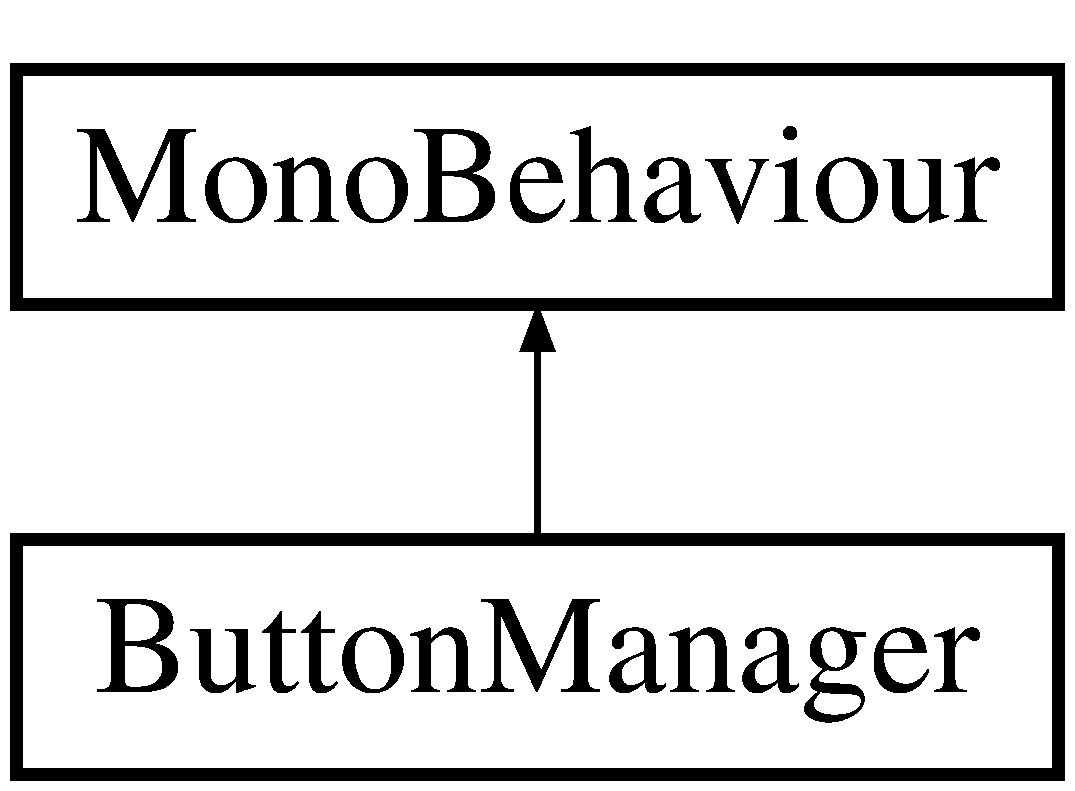
\includegraphics[height=2.000000cm]{class_button_manager}
\end{center}
\end{figure}
\subsection*{Public Member Functions}
\begin{DoxyCompactItemize}
\item 
void \hyperlink{class_button_manager_ace626082f907af4428c5842e9b92a136}{New\+Game\+Btn} (string new\+Game)
\item 
\mbox{\Hypertarget{class_button_manager_a4841ad4fd7809df2ca338169d646f272}\label{class_button_manager_a4841ad4fd7809df2ca338169d646f272}} 
void {\bfseries Exit\+Game\+Btn} ()
\end{DoxyCompactItemize}


\subsection{Detailed Description}
asdfjhalsdkjfhaskdjfhalskdjfhalsdjkf 

\subsection{Member Function Documentation}
\mbox{\Hypertarget{class_button_manager_ace626082f907af4428c5842e9b92a136}\label{class_button_manager_ace626082f907af4428c5842e9b92a136}} 
\index{Button\+Manager@{Button\+Manager}!New\+Game\+Btn@{New\+Game\+Btn}}
\index{New\+Game\+Btn@{New\+Game\+Btn}!Button\+Manager@{Button\+Manager}}
\subsubsection{\texorpdfstring{New\+Game\+Btn()}{NewGameBtn()}}
{\footnotesize\ttfamily void Button\+Manager.\+New\+Game\+Btn (\begin{DoxyParamCaption}\item[{string}]{new\+Game }\end{DoxyParamCaption})}

A test class. A more elaborate class description. 

The documentation for this class was generated from the following file\+:\begin{DoxyCompactItemize}
\item 
Button\+Manager.\+cs\end{DoxyCompactItemize}

\hypertarget{class_flipper_move}{}\section{Flipper\+Move Class Reference}
\label{class_flipper_move}\index{Flipper\+Move@{Flipper\+Move}}
Inheritance diagram for Flipper\+Move\+:\begin{figure}[H]
\begin{center}
\leavevmode
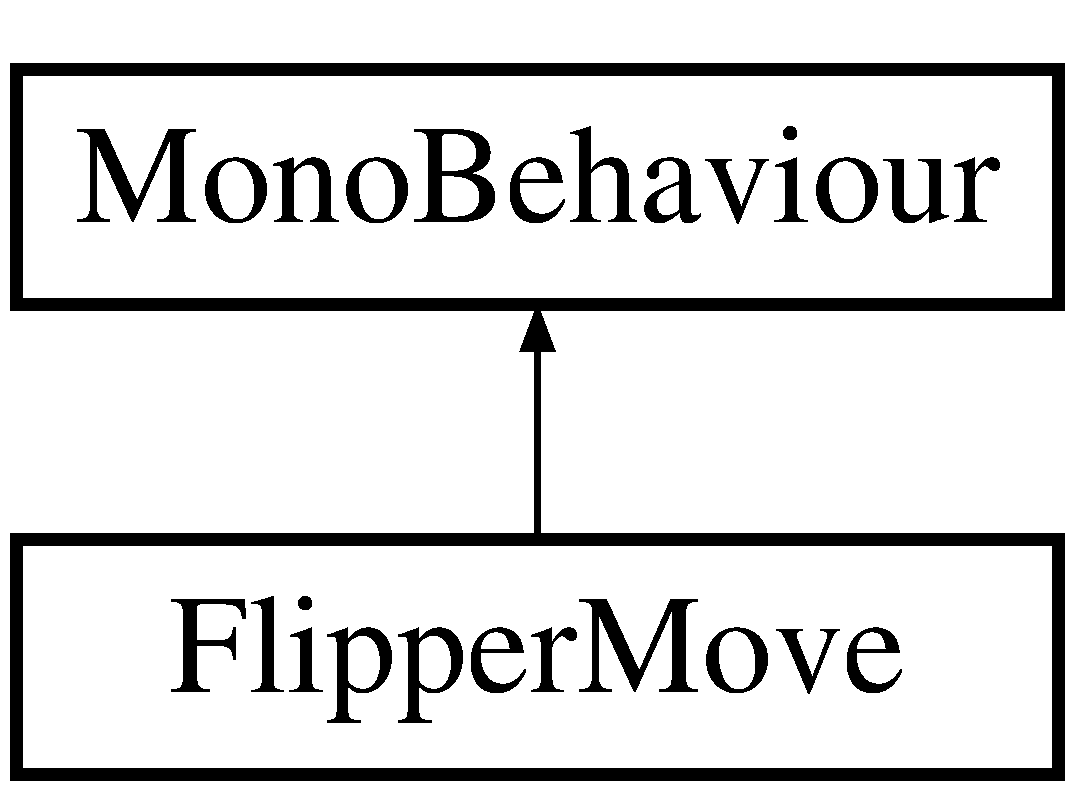
\includegraphics[height=2.000000cm]{class_flipper_move}
\end{center}
\end{figure}
\subsection*{Public Attributes}
\begin{DoxyCompactItemize}
\item 
\mbox{\Hypertarget{class_flipper_move_aa4b8166810663327c8d058822d626387}\label{class_flipper_move_aa4b8166810663327c8d058822d626387}} 
float {\bfseries rest\+Position} = 0f
\item 
\mbox{\Hypertarget{class_flipper_move_a8b35bce53e12f147a1908986f6ffe73f}\label{class_flipper_move_a8b35bce53e12f147a1908986f6ffe73f}} 
float {\bfseries pressed\+Position} = 45f
\item 
\mbox{\Hypertarget{class_flipper_move_a64c20e1451ba300c8d5c9a039b6568b9}\label{class_flipper_move_a64c20e1451ba300c8d5c9a039b6568b9}} 
float {\bfseries hit\+Strength} = 10000f
\item 
\mbox{\Hypertarget{class_flipper_move_a76180542cb57330e4c87225b3e01f50f}\label{class_flipper_move_a76180542cb57330e4c87225b3e01f50f}} 
float {\bfseries flipper\+Damper} = 350f
\item 
\mbox{\Hypertarget{class_flipper_move_a5e3209a830a3bba9f86c3563ed6d2cda}\label{class_flipper_move_a5e3209a830a3bba9f86c3563ed6d2cda}} 
string {\bfseries input\+Name}
\end{DoxyCompactItemize}


The documentation for this class was generated from the following file\+:\begin{DoxyCompactItemize}
\item 
Flipper\+Move.\+cs\end{DoxyCompactItemize}

\hypertarget{class_game_manager}{}\section{Game\+Manager Class Reference}
\label{class_game_manager}\index{Game\+Manager@{Game\+Manager}}
Inheritance diagram for Game\+Manager\+:\begin{figure}[H]
\begin{center}
\leavevmode
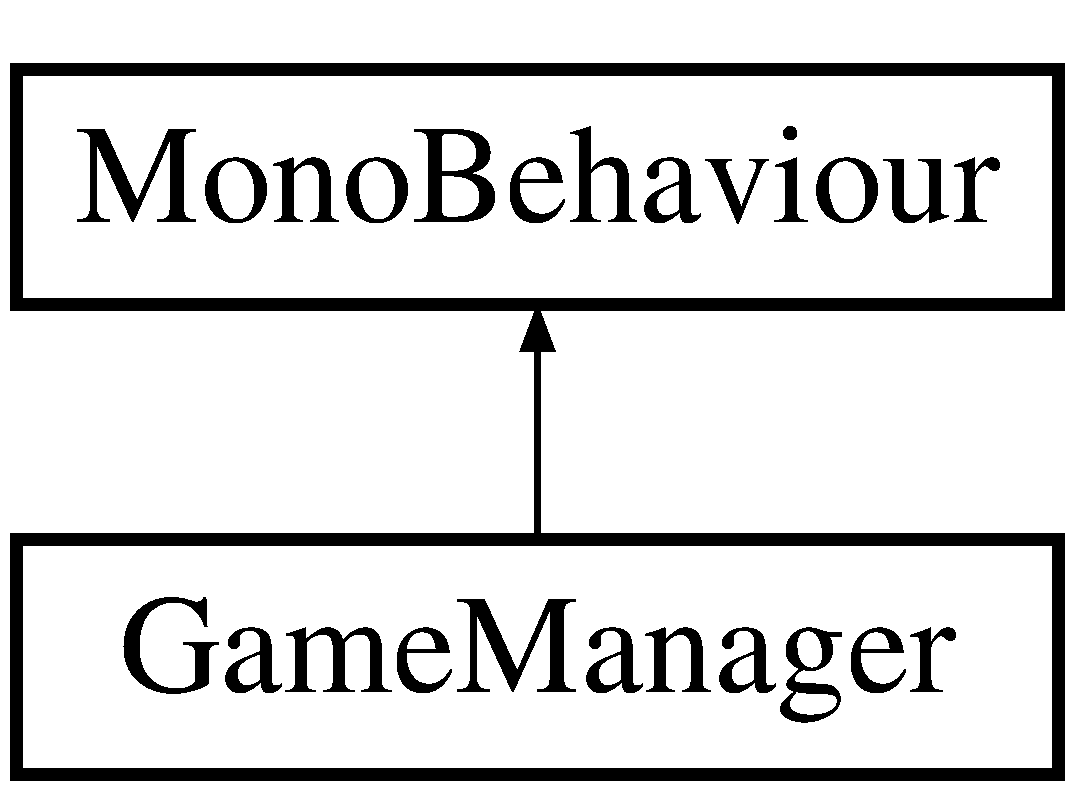
\includegraphics[height=2.000000cm]{class_game_manager}
\end{center}
\end{figure}
\subsection*{Public Attributes}
\begin{DoxyCompactItemize}
\item 
\mbox{\Hypertarget{class_game_manager_a7a3732d88888e672f51ba07d10dc1c2b}\label{class_game_manager_a7a3732d88888e672f51ba07d10dc1c2b}} 
float {\bfseries speed}
\item 
\mbox{\Hypertarget{class_game_manager_ae9711122c3e5251d8f9ff4e02283af09}\label{class_game_manager_ae9711122c3e5251d8f9ff4e02283af09}} 
int {\bfseries score}
\item 
\mbox{\Hypertarget{class_game_manager_a571eb018f12e085310061f8d9128bd70}\label{class_game_manager_a571eb018f12e085310061f8d9128bd70}} 
Game\+Object {\bfseries reset\+Btn}
\item 
\mbox{\Hypertarget{class_game_manager_a398d163978e15786ef9cea1be1c877d9}\label{class_game_manager_a398d163978e15786ef9cea1be1c877d9}} 
Text {\bfseries score\+Text}
\item 
\mbox{\Hypertarget{class_game_manager_aa46bc20b46271084abc755ea0cae7df0}\label{class_game_manager_aa46bc20b46271084abc755ea0cae7df0}} 
Text {\bfseries score\+Text\+Menu}
\item 
\mbox{\Hypertarget{class_game_manager_a1962a62add77291ec291401b94223800}\label{class_game_manager_a1962a62add77291ec291401b94223800}} 
Text {\bfseries best\+Score\+Text}
\item 
\mbox{\Hypertarget{class_game_manager_a81293487e97b92a270eedafff9100b11}\label{class_game_manager_a81293487e97b92a270eedafff9100b11}} 
Layer\+Mask {\bfseries what\+Is\+Ground}
\item 
\mbox{\Hypertarget{class_game_manager_a88384641870110b5d25f42687fe373a7}\label{class_game_manager_a88384641870110b5d25f42687fe373a7}} 
Animator {\bfseries game\+Over\+Anim}
\item 
\mbox{\Hypertarget{class_game_manager_ae73fa16e65d6a73673a2bb11ac272631}\label{class_game_manager_ae73fa16e65d6a73673a2bb11ac272631}} 
Transform {\bfseries contact\+Point}
\end{DoxyCompactItemize}


The documentation for this class was generated from the following file\+:\begin{DoxyCompactItemize}
\item 
Game\+Manager.\+cs\end{DoxyCompactItemize}

\hypertarget{class_ground_points}{}\section{Ground\+Points Class Reference}
\label{class_ground_points}\index{Ground\+Points@{Ground\+Points}}
Inheritance diagram for Ground\+Points\+:\begin{figure}[H]
\begin{center}
\leavevmode
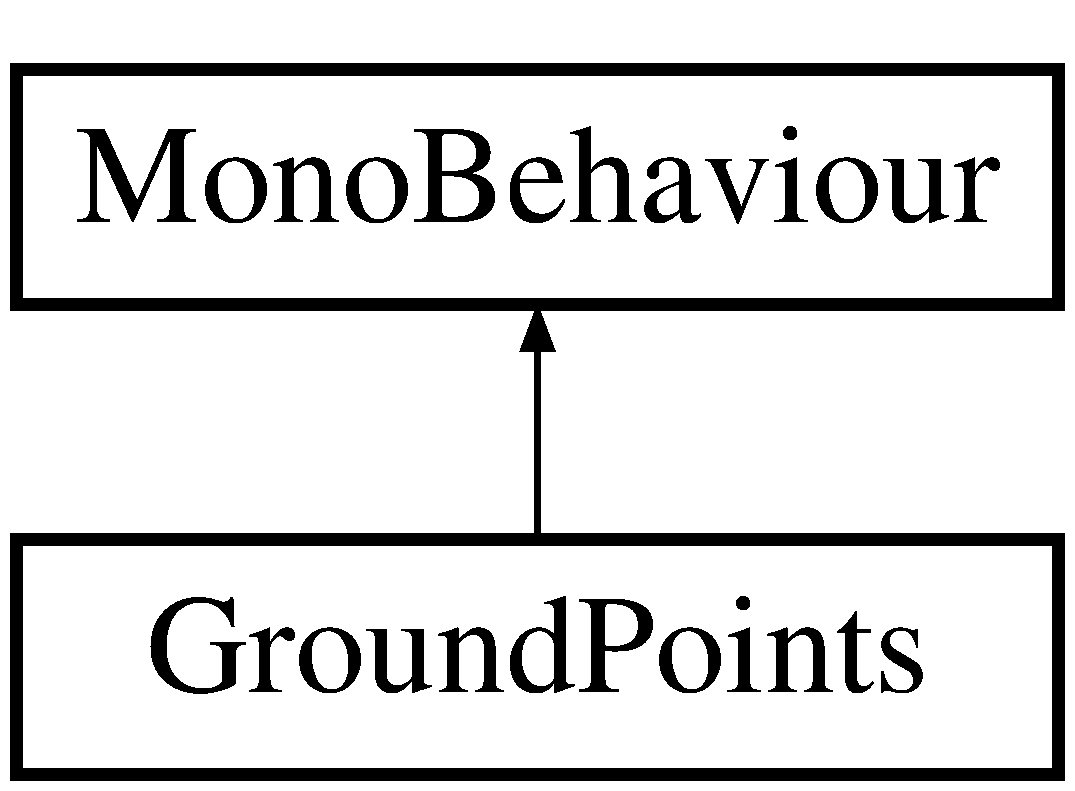
\includegraphics[height=2.000000cm]{class_ground_points}
\end{center}
\end{figure}
\subsection*{Public Attributes}
\begin{DoxyCompactItemize}
\item 
\mbox{\Hypertarget{class_ground_points_aec58fbff5b991b3b14c7a81864e7900b}\label{class_ground_points_aec58fbff5b991b3b14c7a81864e7900b}} 
float {\bfseries score\+Bonus} = 100
\item 
\mbox{\Hypertarget{class_ground_points_ab071f2fc5ced4f16d8ae34d5db534431}\label{class_ground_points_ab071f2fc5ced4f16d8ae34d5db534431}} 
int {\bfseries multiplier} = 1
\item 
\mbox{\Hypertarget{class_ground_points_aae27448239119ba888f51242df8ee807}\label{class_ground_points_aae27448239119ba888f51242df8ee807}} 
int {\bfseries mode} = 0
\end{DoxyCompactItemize}


The documentation for this class was generated from the following file\+:\begin{DoxyCompactItemize}
\item 
Ground\+Points.\+cs\end{DoxyCompactItemize}

\hypertarget{class_obstacle}{}\section{Obstacle Class Reference}
\label{class_obstacle}\index{Obstacle@{Obstacle}}
Inheritance diagram for Obstacle\+:\begin{figure}[H]
\begin{center}
\leavevmode
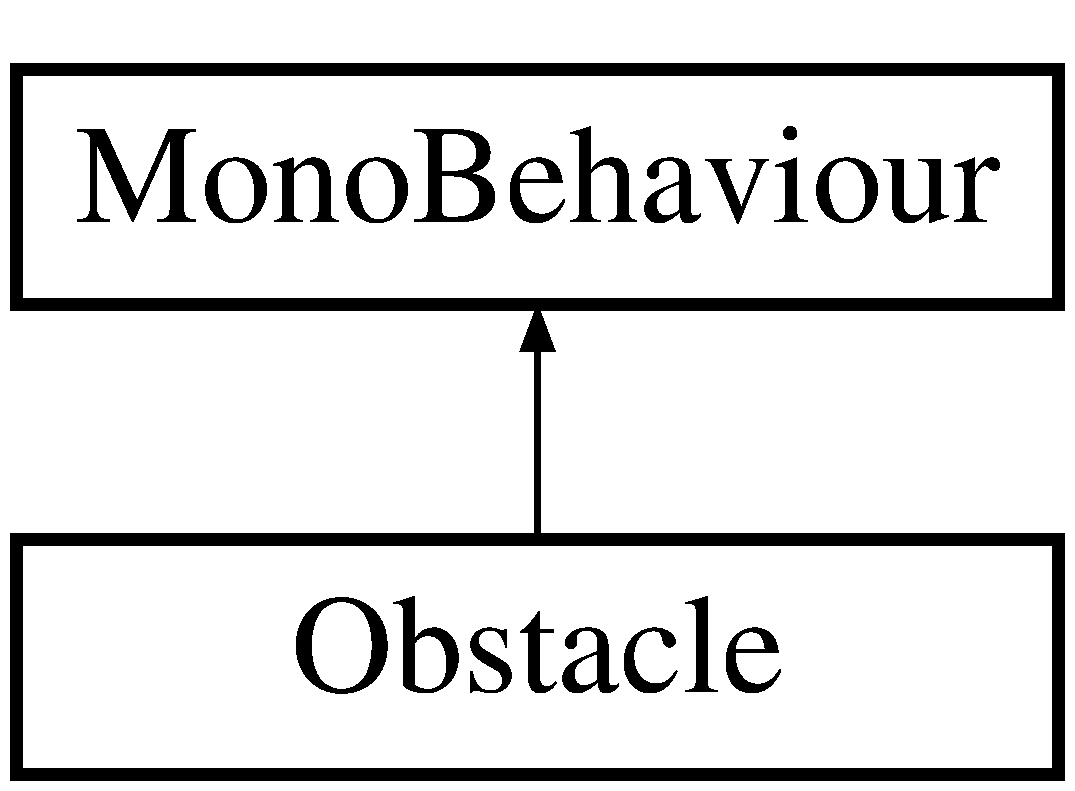
\includegraphics[height=2.000000cm]{class_obstacle}
\end{center}
\end{figure}
\subsection*{Public Attributes}
\begin{DoxyCompactItemize}
\item 
\mbox{\Hypertarget{class_obstacle_ade7caf7691e15d73c3ea585f3440471e}\label{class_obstacle_ade7caf7691e15d73c3ea585f3440471e}} 
int {\bfseries mode} = 0
\item 
\mbox{\Hypertarget{class_obstacle_a7c7ff9b4205e4ec5334d6116ede6c452}\label{class_obstacle_a7c7ff9b4205e4ec5334d6116ede6c452}} 
float {\bfseries score\+Bonus} = 100
\item 
\mbox{\Hypertarget{class_obstacle_a8c31a16efd6da81b7dff1e7be88f84da}\label{class_obstacle_a8c31a16efd6da81b7dff1e7be88f84da}} 
int {\bfseries multiplier} = 1
\end{DoxyCompactItemize}


The documentation for this class was generated from the following file\+:\begin{DoxyCompactItemize}
\item 
Obstacle.\+cs\end{DoxyCompactItemize}

\hypertarget{class_score}{}\section{Score Class Reference}
\label{class_score}\index{Score@{Score}}
Inheritance diagram for Score\+:\begin{figure}[H]
\begin{center}
\leavevmode
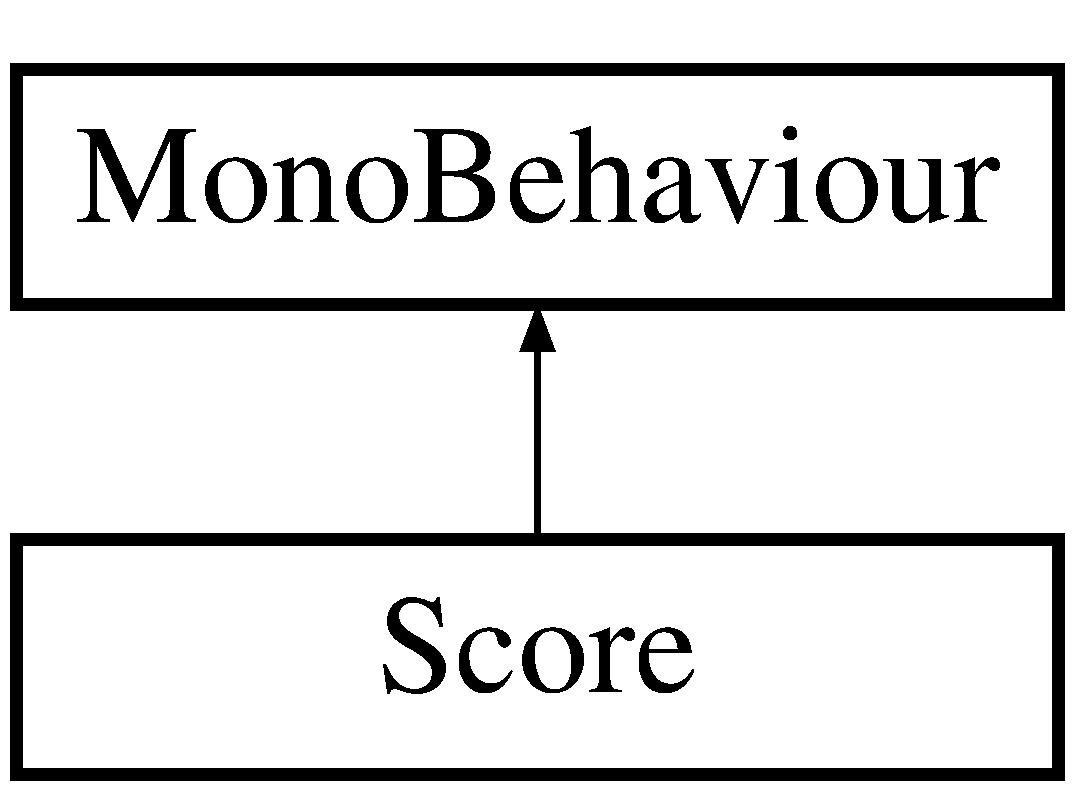
\includegraphics[height=2.000000cm]{class_score}
\end{center}
\end{figure}
\subsection*{Public Attributes}
\begin{DoxyCompactItemize}
\item 
\mbox{\Hypertarget{class_score_a1ddfcf4445cf346df89df41bedd3c714}\label{class_score_a1ddfcf4445cf346df89df41bedd3c714}} 
float {\bfseries high\+Score}
\item 
\mbox{\Hypertarget{class_score_ac4f31ba927c4f661d4fd351cd2ed29f0}\label{class_score_ac4f31ba927c4f661d4fd351cd2ed29f0}} 
s float {\bfseries current\+Score} = 0
\item 
\mbox{\Hypertarget{class_score_a2bd3a3082f332e868fa03bc257a034f4}\label{class_score_a2bd3a3082f332e868fa03bc257a034f4}} 
float \mbox{[}$\,$\mbox{]} {\bfseries top\+Scores}
\end{DoxyCompactItemize}


The documentation for this class was generated from the following file\+:\begin{DoxyCompactItemize}
\item 
Score.\+cs\end{DoxyCompactItemize}

\hypertarget{class_spring}{}\section{Spring Class Reference}
\label{class_spring}\index{Spring@{Spring}}
Inheritance diagram for Spring\+:\begin{figure}[H]
\begin{center}
\leavevmode
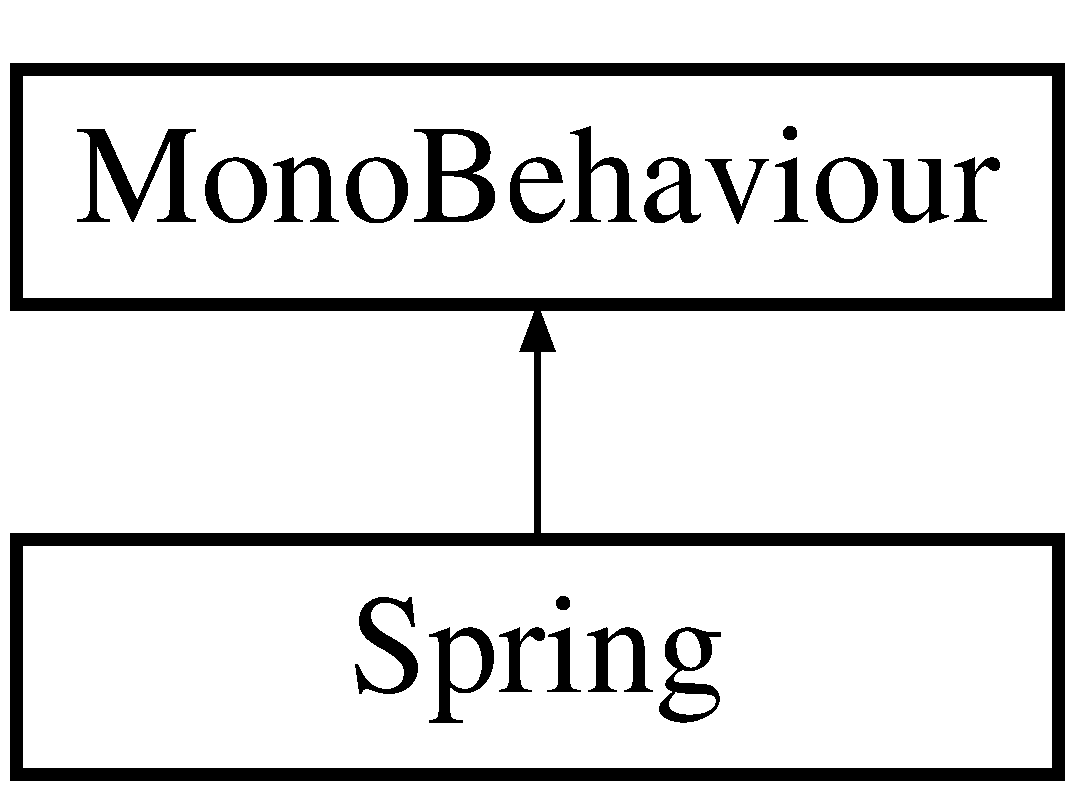
\includegraphics[height=2.000000cm]{class_spring}
\end{center}
\end{figure}
\subsection*{Public Attributes}
\begin{DoxyCompactItemize}
\item 
\mbox{\Hypertarget{class_spring_acaad70263479287c00291512b37f7a65}\label{class_spring_acaad70263479287c00291512b37f7a65}} 
float {\bfseries hit\+Strength} = 50000f
\item 
\mbox{\Hypertarget{class_spring_aa3c6f1b7a112aece7583223d7558be52}\label{class_spring_aa3c6f1b7a112aece7583223d7558be52}} 
float {\bfseries rest\+Position} = 0f
\item 
\mbox{\Hypertarget{class_spring_a7efc825f56da642ad8fa58c7fd46ed13}\label{class_spring_a7efc825f56da642ad8fa58c7fd46ed13}} 
bool {\bfseries wait} = true
\end{DoxyCompactItemize}


The documentation for this class was generated from the following file\+:\begin{DoxyCompactItemize}
\item 
Spring.\+cs\end{DoxyCompactItemize}

%--- End generated contents ---

% Index
\backmatter
\newpage
\phantomsection
\clearemptydoublepage
\addcontentsline{toc}{chapter}{Index}
\printindex

\end{document}
